%!TEX root = ../fbi.tex

\section{Construction of the featureless boson insulator}
\label{sec:fbi}

\begin{figure}
	\centering
	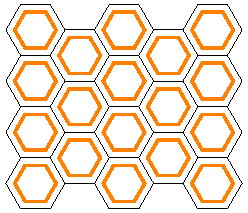
\includegraphics[width=0.6\columnwidth]{fbi3.pdf}
	\caption{Schematic representation of honeycomb FBI}
\end{figure}

In Ref.~\onlinecite{kimchi2013}, Kimchi et al gave an explicit
construction of a bosonic insulator
on the honeycomb lattice that is completely featureless in the bulk.
The state is succinctly described by the following wavefunction:
\begin{equation} \label{eq:def}
\ket{\psi} = \prod\limits_{\varhexagon} \sum\limits_{i \in
\varhexagon} b^{\dagger}_{i} \ket{0}.
\end{equation}
Here, $\varhexagon$ denotes the elementary hexagons of the honeycomb
lattice. We consider two closely related variants of the state, a
version of soft-core bosons where $b_i^\dagger$ creates a boson on
site $i$ and obeys the usual bosonic commutation relations, and a
hard-core version of the same state where $b_i^\dagger$ also creates a
boson but $(b_i^\dagger)^2=0$. In either case, the operator $\sum_{i
\in \varhexagon} b^{\dagger}_{i}$ creates exactly one boson per
hexagon; as there is one hexagon per unit cell of two sites of the
lattice, the state has one boson per unit cell, or half a boson per
site, thus allowing the existence of a featureless state.
In the case of soft-core bosons, the maximum number of bosons
per site is 3.

\bela{Summarize what was calculated in Ref.~\onlinecite{kimchi2013}.}

\subsection{PEPS representation}

In order to make the state~\eqnref{eq:def} more amenable to numerical
simulations, and in particular in order to be able to study its edge
properties, we now derive a representation as a projected entangled
pair states (PEPS). Importantly, this PEPS description will respect
all of the relevant symmetries of \eqnref{eq:def}.

\begin{figure}
	\centering
	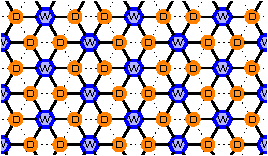
\includegraphics[width=0.8\columnwidth]{FBI_PEPS.pdf}
	\caption{\bela{Make labels math font. I think we might have to
	include physical indices in this figure, maybe very short/thin.}
	Intermediate tensor network for HFBI state. Here, the tensors labeled
	$D$ are located on the sites of the honeycomb lattice, while the
	tensors labeled $W$ are located on the centers of each hexagon.
	Dotted lines thus represent the physical lattice, while the solid
	lines indicate auxiliary bonds over which the tensor network is
	contracted. In this picture, we have suppressed the physical index
	for visual clarity.}
	\label{fig:FBI_PEPS}
\end{figure}

To obtain a PEPS construction, we first choose a local basis $\ket{n}$
of boson occupation numbers, i.e. $b^\dagger b \ket{n} = n \ket{n}$.
The PEPS will thus describe the coefficients of $\ket{\psi}$ in this
basis, $\langle n_1 \ldots n_L | \psi \rangle$. The PEPS
representation is most easily obtained in a two-step construction,
where we first construct the state shown in Fig.~\ref{fig:FBI_PEPS}.
Here, the tensor labeled $W=W^{n_1 \ldots n_6}$, which is placed in
the center of each hexagon, is a rank-6 tensor given by
\begin{equation}
W^{\{n_x\}}  = \left\{ \begin{array}{lr}
													1  : & \sum\limits_x n_x = 1 \\
													0  : & \text{else}
													\end{array} \right. .
\end{equation}
This tensor describes the coefficients of a so-called $W$-state in the
occupation number basis, i.e. $W^{\lbrace n_x\rbrace }= \langle n_1
\ldots n_6 | \sum_{i=1}^6 b_i^\dagger |0\rangle$. We note that this
tensor is symmetric under permutations of its indices.

On the sites of the physical lattice, we have placed a rank-4 tensor
denoted as $D$, shown in panel (a) of Fig.~\ref{fig:FBI_PEPS_2}, which
connects the $W$ tensors from three adjacent hexagons, and as fourth
index has a physical index $p$. For a state of soft-core bosons, where
$p=0,1,2,3$, this tensor is given by
\begin{equation} \label{eqn:D}
D^\mathrm{sc}_{p, i_0 i_1 i_2}  = \left\{ \begin{array}{ll}
													\sqrt{p!}  &: p =i_0+i_1+i_2  \\
													0  &:  \text{else}
													\end{array}
											\right. .
\end{equation}
We can also encode a state of hard-core bosons by replacing $D$ by
\begin{equation}
D^\mathrm{hc}_{p, i_0 i_1 i_2}  = \left\{ \begin{array}{ll}
													1  &: p = i_0+i_1+i_2 \le 1  \\
													0  &:  \text{else}
													\end{array}
											\right.
\end{equation}
Further variants of the state are described in
Appendix ~\ref{Appendix:Variants}.

This tensor network wavefunction manifestly respects all the
translational and point group symmetries of the honeycomb lattice,
since the tensors $W$ and $D$ are invariant under rotations of their
virtual indices in the plane. One can also check that the
wavefunction is $U(1)$ invariant with charge $1$ per plaquette.
\begin{figure}
	\centering
	\subfigure[D tensor]{%
		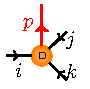
\includegraphics[width=0.18\columnwidth]{D_op.pdf}
		\label{fig:D}
	}
	\quad
	\subfigure[W-tensor and factored form]{%
		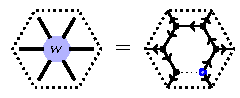
\includegraphics[width=0.5\columnwidth]{w_string.pdf}
		\label{fig:W}
	}
	\subfigure[PEPS tensor network for F.B.I. state]{%
		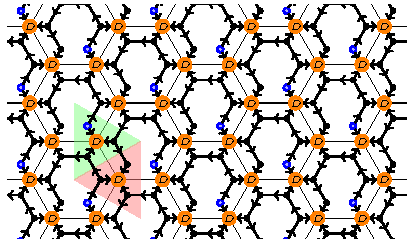
\includegraphics[width=0.8\columnwidth]{FBI_PEPS_2.pdf}
		\label{fig:FBI_PEPS_2A}
	}
\caption{\bela{I think the 1 in the center of the W MPS is confusing. Also, we should have shaded circles showing what the final PEPS tensor is.} Tensors used to put the F.B.I. tensor network in PEPS form. }
\label{fig:FBI_PEPS_2}
\end{figure}

In order to form a PEPS representation with all tensors located on the
vertices, we first factor the $W$-tensor into a matrix-product state
of six tensors as shown in panel (b) of Fig.~\ref{fig:FBI_PEPS_2}. We
choose a form of the MPS that breaks the rotational symmetry
of the W-state (which appears as translational symmetry of the MPS).
This allows us to obtain an MPS description with a small bond dimension
of $M=2$; a fully symmetric choice would require bond dimension 6.
Since these states are physically equivalent, we expect all
gauge-invariant quantities to be unaffected by this choice.
The decomposition is given by
\begin{equation}
W^{i_1 i_2 i_3 i_4 i_5 i_6} = \sum\limits_{\alpha_1 \ldots \alpha_5} V^{i_1}_{\alpha_1} W^{i_2}_{\alpha_1 \alpha_2}
%W^{i_3}_{\alpha_2 \alpha_3} W^{i_4}_{\alpha_3 \alpha_4}
\ldots
W^{i_5}_{\alpha_4 \alpha_5} X^{i_6}_{\alpha_5}
\end{equation}
where $V^{i_1}_{\alpha_1} = \delta_{i_1, \alpha_1}$, $X^{i_6}_{\alpha_5} = \delta_{i_6,\alpha_5+1}+\delta_{i_6,\alpha_5-1}$, and
\begin{equation*}
W_{i_0 i_1}^{j}  = \left\{ \begin{array}{ll}
													1  &:  i_0+j=i_1 \\
													0  &:  \text{else}
													\end{array}
											\right.,
\end{equation*}
where each index takes values in $\{0, 1\}$. Applying this to each
$W$-tensor yields the state as shown in panel (c) of
Fig.~\ref{fig:FBI_PEPS_2}. By contracting the three tensors in each
shaded region together, we obtain a PEPS in the regular form as shown
in Fig.~\ref{fig:PEPS}. The resulting PEPS has a bond dimension of
$M=2$ on the horizontal bonds, and a bond dimension of $M=4$ on all
other bonds. While it superficially breaks
the rotational symmetry of the lattice, it is an exact representation
of the FBI state and does not break any symmetries after contracting
the indices.

This decomposition respects the physical U(1) charge conservation
symmetry in that all tensors are separately
U(1)-invariant~\cite{bauer2011}. To make this manifest, we have
indicated in Fig.~\ref{fig:FBI_PEPS_2} arrows on each bond that show
the flow of charge.

\subsection{Representation on infinite cylinders}
For the calculations presented in this manuscript, we consider the
state $\ket{\psi}$ on a cylinder of infinite length, but finite
circumference $L$. In Fig.~\ref{fig:PEPS}, we have indicated the
choice of boundary conditions for the cylinder. For many practical
purposes, the PEPS on an infinite cylinder can be represented as an
infinite, translationally invariant matrix-product state of bond
dimension $2^L$.

\begin{figure}
	\centering
	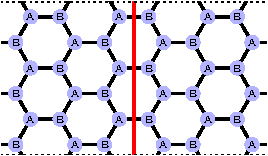
\includegraphics[width=\columnwidth]{Hex_PEPS.pdf}
	\caption{\bela{In this picture, we need to indicate the physical
	legs (maybe in a different color).} Pictoral representation of a
	PEPS on a honeycomb lattice. The tensors A and B are rank 4, with
	the physical leg at each site not shown for visual clarity. By
	gluing together the top and bottom edge of this picture, we get the
	"zig-zag" cylinder configuration used for most of the calculations
	in this paper. This cylinder is 3 unit cells wide, so we will call
	it the L=3 cylinder. In section \ref{sec:ES}, we will study the
	entanglement cut specified by the red line for various cylinder
	widths.}
	\label{fig:PEPS}
\end{figure}
